% LTeX: language=de-CH

\section{Ergebnisse} \label{sec:ergebnisse}

\subsection{Beschreibung des Datensatzes}

\subsubsection{Soziodemografische Merkmale der Stichprobe}

Die Stichprobe des Probelaufs umfasst insgesamt 24 Personen. Die Mehrheit gehört der Altersgruppe \emph{16–25 Jahre} an (n = 20; 80\,\%). Nur wenige Personen entfallen auf die Gruppen \emph{26–35 Jahre} (n = 3; 12\,\%) und \emph{56–65 Jahre} (n = 1; 4\,\%); eine Person machte keine Altersangabe.

Bezüglich des \emph{sozialen Geschlechts} gaben 15 Personen (60\,\%) an, \emph{Mann} zu sein, 9 Personen (36\,\%) identifizierten sich als \emph{Frau}, und eine Person (4\,\%) als \emph{trans Mann}. Als biologisches Geschlecht gaben 16 Personen (64\,\%) an, \emph{männlich} zu sein, 8 (32\,\%) an, \emph{weiblich} zu sein, eine Person machte keine Angabe.

Die \cref{tab:kreuztabelle_abs} zeigt die Verteilung von sozialem Geschlecht und Altersgruppe (absolute Häufigkeiten).

\begin{table}[H]
    \centering
    \caption{Kreuztabelle: Soziales Geschlecht und Altersgruppe (absolute Häufigkeiten)}
    \label{tab:kreuztabelle_abs}
    \begin{tabular}{lccccc}
    \toprule
    \textbf{Geschlecht} & 16--25 & 26--35 & 56--65 & Keine Angabe & Gesamt \\
    \midrule
    Mann       & 12 & 2 & 0 & 1 & 15 \\
    Trans Mann &  0 & 0 & 1 & 0 & 1  \\
    Frau       &  8 & 1 & 0 & 0 & 9  \\
    \midrule
    \textbf{Gesamt} & 20 & 3 & 1 & 1 & 25 \\
    \bottomrule
    \end{tabular}
\end{table}

Weitere soziodemografische Merkmale der Teilnehmenden umfassen u.\,a. sexuelle Orientierung, Bildungsstand, Erwerbsstatus, Haushaltseinkommen, Haushaltsstruktur und -finanzierung, sowie Erfahrungen mit Diskriminierung. Eine vollständige Übersicht über die Verteilung dieser Merkmale findet sich in \cref{sec:appendix_demographics}.


\subsubsection{Beschreibung der erfassten Momentaufnahmen}

Im Rahmen der Pilotstudie wurden insgesamt 106 Momentaufnahmen erhoben, verteilt auf die 25 Teilnehmenden. Die Anzahl abgeschlossener Befragungen pro Person variierte dabei erheblich (\textit{M} = 4{,}2; \textit{SD} = 2{,}9; \textit{Min} = 1; \textit{Max} = 12), was auf eine ungleichmässige Nutzung der App innerhalb der Teilnehmendengruppe hinweist (siehe \cref{fig:survey_counts}).

Die Tätigkeiten, die während der Beantwortung der Umfrage durchgeführt wurden, decken ein breites Spektrum ab. Am häufigsten gaben Teilnehmende an, zu arbeiten oder zu studieren (n = 48, 43\,\%), gefolgt von Freizeit- und Entspannungsaktivitäten (n = 19, 22\,\%) und Reisen bzw. Pendeln (n = 9, 10\,\%). Weitere Angaben umfassten etwa Kochen, Medienkonsum, soziale Aktivitäten oder Kombinationen mehrerer Aktivitäten.

Bezüglich des Aufenthaltsortes befanden sich die meisten Personen zum Zeitpunkt der Umfrage entweder an einer Bildungsinstitution (n = 38, 35\,\%) oder zu Hause (n = 28, 27\,\%). Weitere häufig genannte Orte waren unterwegs zu Fuss, per Fahrrad oder im Auto (n = 11, 11\,\%), öffentliche Verkehrsmittel (n = 8, 7\,\%) sowie die Wohnung anderer Personen oder Parks und Grünflächen (vgl. \cref{app:location_table}). Die Aufenthaltsorte verteilten sich dabei nahezu gleichmässig auf Innenräume (n = 54, 51\,\%) und Aussenräume (n = 52, 49\,\%).

Auch die soziale Situation während der Umfrage war sehr unterschiedlich: Ein Drittel der Momentaufnahmen wurde allein durchgeführt (n = 37, 35\,\%), ein weiteres Drittel in Gegenwart von Freund*innen (n = 28, 26\,\%). Weitere häufige Angaben betrafen die Anwesenheit von Fremden (n = 10, 9\,\%), Kolleg*innen (n = 8, 8\,\%) oder verschiedenen Kombinationen dieser Gruppen (vgl. \cref{app:people_table}).

Diese Vielfalt an Tätigkeiten, Kontexten und sozialen Situationen zeigt das Potenzial des Erhebungsinstruments, subjektives Wohlbefinden in unterschiedlichen Alltagssituationen ökologisch valide zu erfassen.



\begin{figure}[htbp]
    \centering
    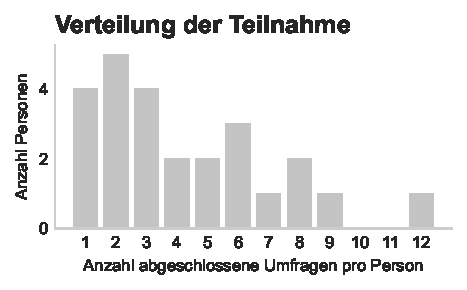
\includegraphics[width=8cm]{analysis/plots/survey_counts.pdf}
    \caption{Aufteilung nach Anzahl abgeschlossener Umfragen pro Person}
    \label{fig:survey_counts}
\end{figure}




\subsubsection{Umfang und demografische Merkmale}

\subsubsection{Qualitative Rückmeldungen der Teilnehmenden}

\subsection{Intersektionale Analysen am erhobenen Material}

\subsubsection{Exemplarische Analysen mittels MAIHDA}
\label{sec:pilot_maihda}

In einem Probelauf wurde geprüft, ob die vorliegenden Daten eine intersektionale Multilevel-Analyse nach dem \gls{maihda}-Ansatz zulassen. Konkret sollte untersucht werden, ob (a) genügend Beobachtungen je intersektionalem Stratum vorhanden sind und (b) die zwischenstratale Varianz gross genug ist, um stabile Random-Effects-Schätzungen zu erhalten.

\paragraph{Iterative Spezifikation der Strata}
Ausgangspunkt war ein Set über alle erhobenen Achsen: Biologisches Geschlecht, Soziales Geschlecht, Sexuelle Orientierung, Ausbildungsstufe, Gruppiertes Äquivalenz-Einkommen, Anstellungsverhältnis, Geburtsland, Vorhandene Behinderungen.

Die Kombination dieser Merkmale ergab 20 unterschiedliche Strata. Die Zellgrössen (Anzahl Personen pro Stratum) sind allerdings sehr klein (siehe \cref{tab:zellgroessen_alle_achsen}).

\begin{table}[h]
    \centering
    \begin{tabular}{rl}
        count & 20 \\
        mean & 1.25 \\
        std & 0.55 \\
        min & 1 \\
        max & 3 \\
    \end{tabular}
    \caption{Zellgrössen pro Stratum mit allen Achsen}
    \label{tab:zellgroessen_alle_achsen}
\end{table}

Mit diesem Set von Strata ist die Modellierung nicht möglich, da die Zellgrössen zu klein sind und eine gute Schätzung der Varianzanteile nicht möglich ist.

Um die Modellierbarkeit zu erhöhen, wurde das Stratum anschliessend auf zwei theoretisch zentrale Achsen reduziert: Biologisches Geschlecht und Alter.

Dies führte zu insgesamt $6$ Strata, mit folgenden Zellgrössen:

\begin{table}[h]
    \centering
    \begin{tabular}{rl}
        count & 6 \\
        mean & 4.17 \\
        std & 4.7 \\
        min & 1 \\
        max & 12 \\
    \end{tabular}
    \caption{Zellgrössen pro Stratum mit reduzierten Achsen}
    \label{tab:zellgroessen_reduzierte_achsen}
\end{table}

Auch hier gibt es noch einzelne Strata mit weniger als 3 Beobachtungen.

\begin{table}[h]
    \centering
    \begin{tabular}{lll}
        Gender & Altersgruppe & Anzahl \\
        \hline
        man & 16 – 25 & 2 \\
        trans man & 56 – 65 & 1 \\
        man & missing & 1 \\
        woman & 26 – 35 & 1 \\
    \end{tabular}
    \caption{Strata mit weniger als 3 Beobachtungen}
    \label{tab:zellgroessen_reduzierte_achsen}
\end{table}

Trotzdem wurde versucht, mit diesem Set von Strata eine MAIHDA-Analyse durchzuführen.

Für jedes kontinuierliche Outcome (\texttt{sense\_of\_belonging}, \texttt{environmen\_pleasure}, \texttt{environment\_lively}, \texttt{environment\_nature}, \texttt{environment\_noise}) wurde ein zweistufiges MAIHDA-Setting geschätzt:
\begin{description}
    \item[Modell~1A (Nullmodell):] Zufallsinterzept auf Stratum-Ebene, keine festen Effekte der Achsen.
    \item[Modell~1B (Additives Modell):] Zusätzlich feste Haupteffekte von \texttt{age\_group} und \texttt{gender}; der verbleibende Stratum-Random-Effect wird als Interaktionsanteil interpretiert.
\end{description}
Aufgrund der geringen Zellgrössen wurde kein zusätzlicher Random-Intercept auf Personenebene modelliert. Die Schätzung erfolgte mittels \texttt{statsmodels.mixedlm} (MLE, Optimierer \texttt{lbfgs}).


\subsection{Varianzzerlegung (VPC, PCV)}
Die geschätzten Varianzanteile zwischen Strata (Variance Partition Coefficient, VPC) waren durchgängig extrem klein. Beispielhaft:

\begin{center}
\begin{tabular}{lrrrr}
\toprule
Outcome & VPC$_{\text{Null}}$ & VPC$_{\text{add}}$ & PCV & $n$ (Zeilen) \\
\midrule
\texttt{sense\_of\_belonging}      & $1.24\times 10^{-5}$ & $1.15\times 10^{-6}$ & 90.7\% & 106 \\
\texttt{environmen\_pleasure}      & $\approx 0$          & $4.40\times 10^{-7}$ & --      & 106 \\
\texttt{environment\_lively}       & $2.95\times 10^{-4}$ & $3.43\times 10^{-5}$ & 88.2\%  & 106 \\
\texttt{environment\_nature}       & $1.03\times 10^{-2}$ & $1.12\times 10^{-6}$ & 99.99\% & 106 \\
\texttt{environment\_noise}        & $1.95\times 10^{-2}$ & $2.98\times 10^{-5}$ & 99.85\% & 106 \\
\bottomrule
\end{tabular}
\end{center}

Die nahezu Null liegenden VPCs belegen, dass (a) die Outcomes sich zwischen den Strata kaum unterscheiden und (b) die Stratum-Varianz im Modell auf Null \emph{geschrumpft} wird. PCV-Werte sind bei einem praktisch Null-VPC im Nullmodell numerisch instabil (z.\,B.\ negative oder extrem grosse Werte) und daher nicht interpretierbar.

\subsection{Schlussfolgerung}
Die Pilotanalyse zeigt, dass mit den vorliegenden Daten keine sinnvolle MAIHDA-Varianzzerlegung durchführbar ist. Gründe:
\begin{enumerate}
    \item \textbf{Zu kleine Strata-Zellgrössen}: Die meisten Strata enthalten nur eine Person bzw.\ sehr wenige Beobachtungen.
    \item \textbf{Geringe zwischenstratale Varianz}: Die betrachteten Outcomes variieren kaum zwischen den (reduzierten) Strata.
    \item \textbf{Numerische Instabilität}: Die Random-Effects-Kovarianzmatrix wird singular; die Schätzung kollabiert auf Randlösungen.
\end{enumerate}

\paragraph{Implikation für die weitere Analyse.}
Für die Beantwortung der Forschungsfrage (Einfluss situativer Umweltfaktoren auf affektives Wohlbefinden) bietet es sich an, die Umweltvariablen als Level-1-Prädiktoren in einem vereinfachten Modell (z.\,B.\ lineares Modell mit cluster-robusten Standardfehlern nach Person oder ein Mixed Model nur mit Personen-Random-Intercept) zu analysieren. Intersectionale Unterschiede können vorerst über feste Effekte (z.\,B.\ \texttt{C(age\_group)}, \texttt{C(gender)}) kontrolliert werden. Eine vollwertige MAIHDA-Anwendung ist erst mit grösserer Stichprobe und ausreichenden Zellgrössen pro Stratum sinnvoll.

\subsubsection{Illustration möglicher Zusammenhänge zwischen Umwelt und Wohlbefinden}

\subsection{Interpretation der explorativen Befunde}


